\documentclass{article}
\usepackage{background}
\backgroundsetup{scale=2,angle=0,opacity=0.1,contents={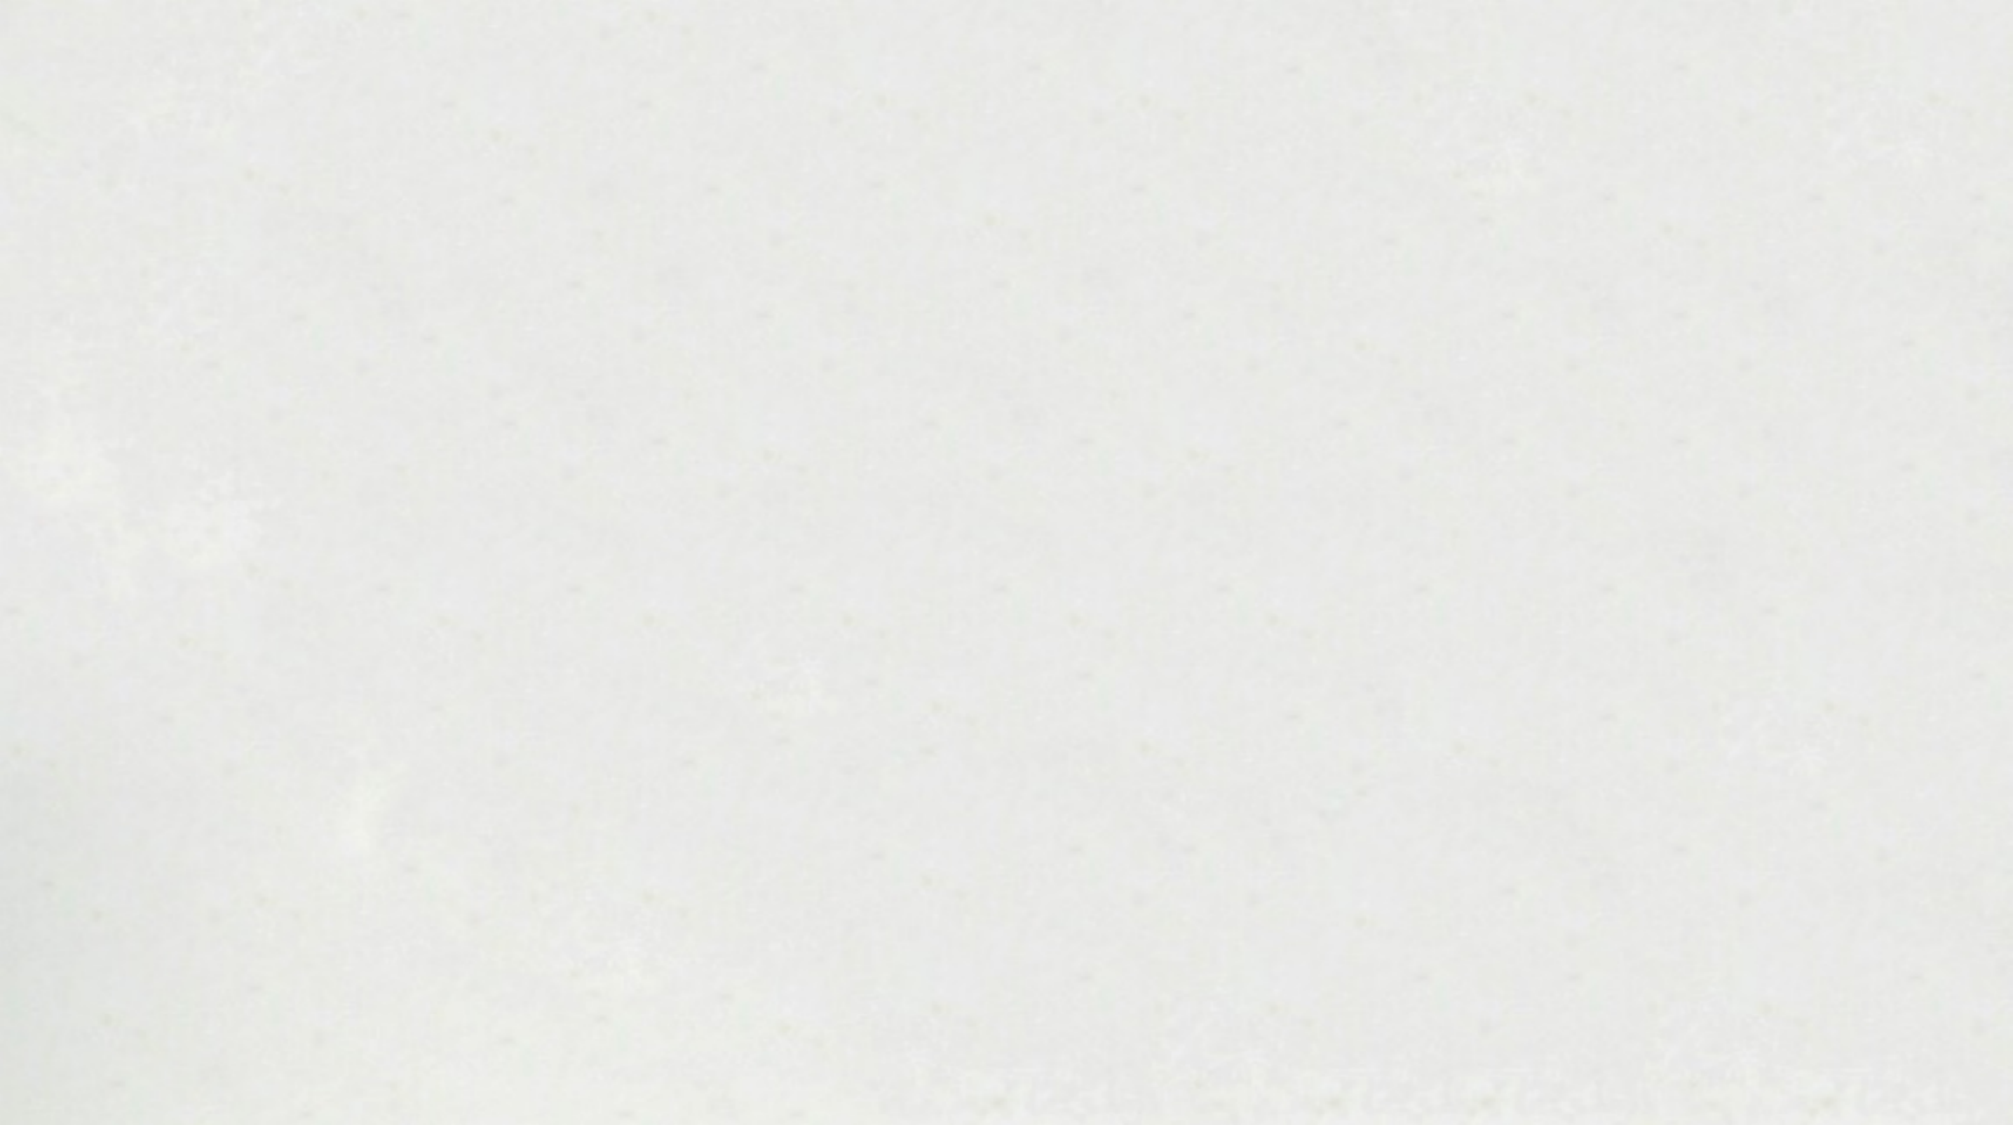
\includegraphics[width=\paperwidth, height=\paperwidth, keepaspectratio]{Picture1.png}}}
\usepackage[UTF8]{ctex}
\usepackage{amsmath}
\begin{document}




\noindent $$T(n) = 2T(\frac{n}{2}) + \Theta(n)$$
$$\Theta(n\log{n})$$

$$A(x) = a_0 + a_1x + a_2x^2 + ... + a_{n-1}x^{n-1}$$
$$A^{[0]}(x) = a_0 + a_2x + a_4x^2 + ... + a_{n-2}x^{\frac{n}{2}-1}$$
$$A^{[1]}(x) = a_1 + a_3x + a_5x^2 + ... + a_{n-1}x^{\frac{n}{2}-1}$$
$$\Downarrow$$
$$A^{[0]}(x^2) = a_0 + a_2x^2 + a_4x^4 + ... + a_{n-2}x^{n-2}$$
$$xA^{[1]}(x^2) = a_1x + a_3x^4 + a_5x^5 + ... + a_{n-1}x^{n-1}$$


$$A(x) = A^{[0]}(x^2) + x A^{[1]}(x^2)$$
$$A(\omega^k_n) = A^{[0]}((\omega^k_n)^2) + \omega^k_n A^{[1]}((\omega^k_n)^2)$$
$$A(\omega^{k + \frac{n}{2}}_n) = A^{[0]}((\omega^{k + \frac{n}{2}}_n)^2) + \omega^{k + \frac{n}{2}}_n A^{[1]}((\omega^{k + \frac{n}{2}}_n)^2)$$
$$(\omega^{k + \frac{n}{2}}_n)^2 = (\omega^k_n)^2 = \omega^k_{\frac{n}{2}}$$
$$\omega^{k + \frac{n}{2}}_n = -\omega^{k}_{n}$$
$$\Downarrow$$
$$A(\omega^k_n) = A^{[0]}(\omega^k_{\frac{n}{2}}) + \omega^k_n A^{[1]}(\omega^k_{\frac{n}{2}})$$
$$A(\omega^{k + \frac{n}{2}}_n) = A^{[0]}(\omega^k_{\frac{n}{2}}) - \omega^{k}_n A^{[1]}((\omega^{k}_{\frac{n}{2}})$$
消去引理:$$\omega^{dk}_{dn} = \omega^k_n$$
$$proof.\omega^{dk}_{dn} = (e^{\frac{2\pi}{dn}i})^{dk}= (e^{\frac{2\pi}{n}i})^k=\omega^k_n$$
折半引理:$$(\omega^{k+\frac{n}{2}}_n)^2 = (\omega^k_n)^2 = \omega^k_{\frac{n}{2}}$$
$$proof. \omega^{k + \frac{n}{2}}_n = \omega^k_n\omega^{\frac{n}{2}}_n = -\omega^k_n, (\omega^k_n)^2 = \omega^{2k}_n = \omega^k_{\frac{n}{2}}$$

\textbf{n次单位复数根}是满足$\omega^n=1$的复数$\omega$。$n$次单位复数根恰好有n个: 对于$k=0,1,...,n-1$,这些根是$e^{\frac{2\pi ik}{n}}$\\
欧拉公式:
    $$e^{iu}=cos(u)+isin(u)$$
值$\omega_n=e^{\frac{2\pi i}{n}}$称为\textbf{主$n$次单位根}

根据霍纳法则,我们可以在$\Theta(n)$的时间复杂度内完成求值运算:  
$$A(x_0) = a_0+x_0(a_1+x_0(a_2+...+x_0(a_{n-2}+x_0(a_{n-1}))...))$$

而如果某个凸集A有两个凸包M1与M2,则$M1 \bigcap M2$也能盖住凸集A,且$M1 \bigcap M2 \subset M1$,但M1是A的凸包,故$ M1 \subset M1 \bigcap M2$,故$M1 \bigcap M2 = M1$.同理$M1 \bigcap M2 = M2$.即$M1 = M2$
由于全平面是一个凸集,故任何平面点集都可用全平面盖住,即能被凸集盖住,从而盖住该凸集的所有凸集的交集存在,即凸包存在. \\
\noindent DFT  

\noindent 我们希望计算次数界为n的多项式  
$$A(x) = \sum^{n-1}_{j=0}a_jx^j$$
在$\omega^0_n,\omega^1_n,\omega^2_n,...,\omega^{n-1}_n$处的值(即在$n$个$n$次单位复数根处)。假设A以系数形式给出:$a = (a_0,a_1,a_2,...,a_{n-1})$。接下来对$k=0,1,...,n-1$,定义结果$y_k$:
$$y_k=A(\omega^k_n)=\sum^{n-1}_{j=0}a_j\omega^{kj}_{n}$$
向量$y=(y_0,y_1,...,y_{n-1})$就是系数向量$a = (a_0,a_1,a_2,...,a_{n-1})$的\textbf{离散傅里叶变换}。
\par 对于 $\forall$ x, y $\in$ C 与 $\forall$  $\lambda\in \lbrack 0, 1 \rbrack $ ,有
$\lambda x + (1-\lambda)y \in C$
$$
\left|
\begin{matrix}
x_1 & y_1 & 1 \\
x_2 & y_2 & 1 \\
x_3 & y_3 & 1 \\
\end{matrix}
\right| = x_1y_2+x_3y_1+x_2y_3-x_3y_2-x_2y_1-x_1y_3
$$

$\mathcal{O}(n\log{}n)$
$\mathcal{M}(n\log{}n)$
\emph{mx}

FFT(a, \emph{lim}):

  \qquad if \emph{lim} == 1 return

  \qquad $a^{[0]} = (a_0,a_2,...,a_{n-2})$

  \qquad $a^{[1]} = (a_1,a_3,...,a_{n-1})$  

  \qquad FFT($a^{[0]}$,\emph{lim}>>1)  

  \qquad FFT($a^{[1]}$,\emph{lim}>>1)  

  \qquad $\omega_n = e^{\frac{2\pi}{n}i} = cos(\frac{2\pi}{n}) + isin(\frac{2\pi}{n})$  

  \qquad $\omega$ = 1  

  \qquad for k = 0 .. $\frac{n}{2} -1$  

      \qquad\qquad $a_k = a^{[0]}_k + \omega a^{[1]}_k$  

      \qquad\qquad $a_{k+\frac{n}{2}} = a^{[0]}_k - \omega a^{[1]}_k$  

      \qquad\qquad $\omega = \omega\omega_n$  



\newpage



\end{document}

